\chapter{Dokumentacja użytkowa}
W poniższym rozdziale zostanie zaprezentowana dokumentacja użytkowa aplikacji wytworzonej na potrzeby projektu.\ W dokumentacji zostaną zaprezentowane poszczególne ekrany oraz interakcje.


\section{Logowanie}
Ekran logowania to pierwszy ekran widoczny dla użytkownika niezalogowanego do systemu.\ Tak jak wskazano na \refsource{rysunku}{fig:log} na ekranie występuje prosty formularz pozwalający na wpisanie loginu i hasła użytkownika w celu weryfikacji tożsamości logowanego.\ Po wciśnięciu przycisku ''\textit{Zaloguj się}'' użytkownik zostaje przekierowany do swojego profilu.\ W przypadku błędnych danych uwierzytelniających użytkownik otrzyma komunikat zwrotny tak jak na \refsource{rysunku}{fig:badlog}.

\begin{figure}[H]
    \centering
    \begin{subfigure}[b]{0.4\textwidth}
        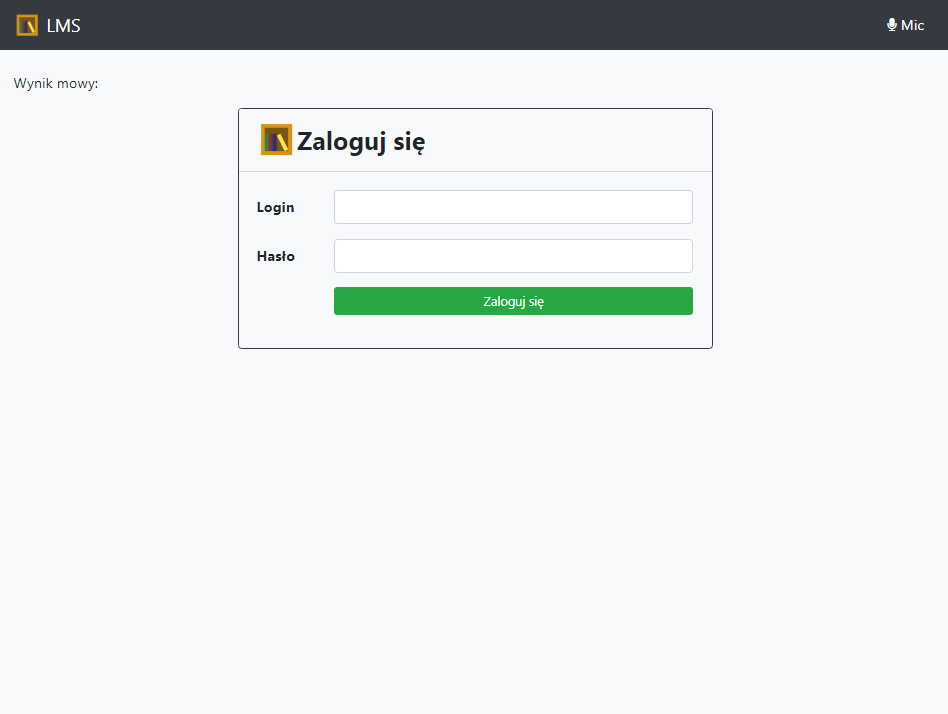
\includegraphics[width=\textwidth]{images/login}
        \captionsource{Ekran logowania}{Opracowanie własne}
        \label{fig:log}
    \end{subfigure}
    \hfill
    \begin{subfigure}[b]{0.4\textwidth}
        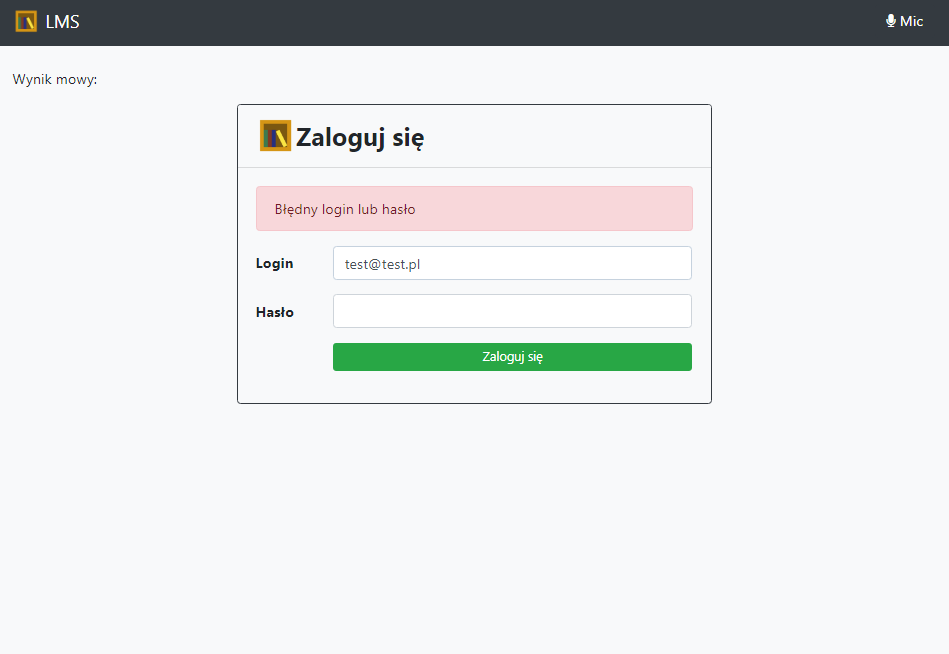
\includegraphics[width=\textwidth]{images/badlogin}
        \captionsource{Ekran logowania - błędne dane}{Opracowanie własne}
        \label{fig:badlog}
    \end{subfigure}
    \captionsource{Logowanie}{Opracowanie własne}
    \label{fig:book-ccccc}
\end{figure}

Po zalogowaniu, użytkownik przechodzi do ekranu głównego, który jednocześnie jest ekranem ukazującym ogólne statystyki.\ Został on ukazany na \refsource{rysunku}{fig:das}

\begin{figure}[H]
    \centering
    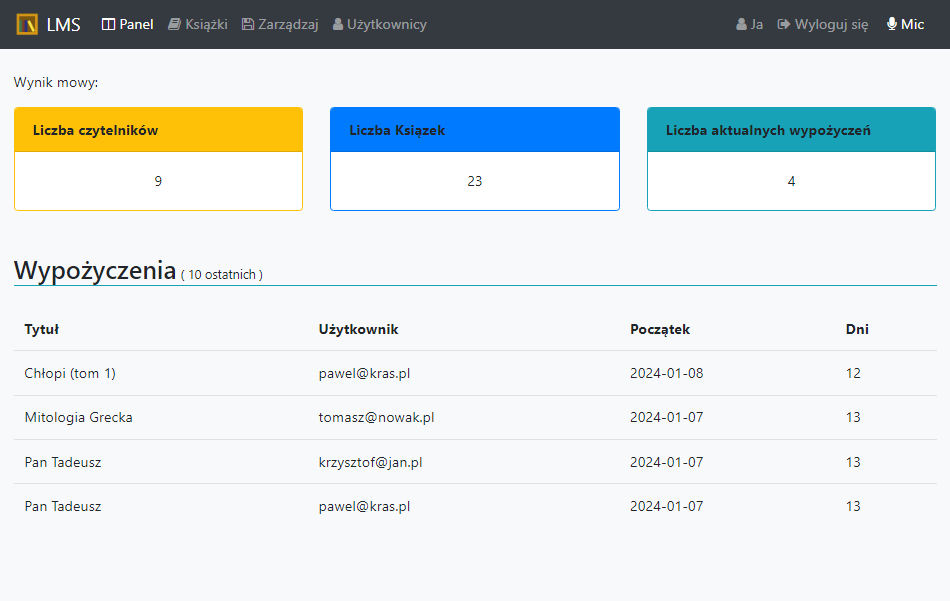
\includegraphics[width=\textwidth]{images/first}
    \captionsource{Ekran początkowy}{Opracowanie własne}
    \label{fig:das}
\end{figure}

Na ekranie zostały zaprezentowane takie informacje jak:
\begin{itemize}
    \item liczba czytelników
    \item liczba książek
    \item liczba aktualnych wypożyczeń
    \item ostatnie 10 wypożyczeń
\end{itemize}
Pozwala to użytkownikowi zorientować się w aktualnej sytuacji biblioteki.

W górnym prawym rogu ekranu dostępna jest ikona mikrofonu, po któej przyciśnięciu aplikacja nasłuchuje wydawanych komend.\ Po wypowiedzeniu nazwy zakładki z górnego paska użytkownik zostanie do niej przekierowany.


\section{Książki}
Ekran ''\textit{Książki}'' pozwala na zarządzanie zbiorem książek.\ Pierwszy ekran pozwala podejrzeć cały zbiór oraz wyszukiwać konkretne tytuły.\ Dodatkowo z tego okna można przejść na zakładkę informacyjną książki, oraz dodać nową pozycję.\ Na tym ekranie po włączeniu opcji \textit{mikrofonu}, można dodać nową książkę bądź wybrać konkretny tytuł.\ Aby wybrać tytuł należy powiedzieć słowo ''\textit{Książka}'', a następnie powiedzieć tytuł książki.\ Działanie ekranu zostało przedstawione na \textbf{rysunkach}~\textbf{\ref{fig:book}}~\textbf{\ref{fig:book1}}.

\begin{figure}[H]
    \centering
    \begin{subfigure}[b]{0.4\textwidth}
        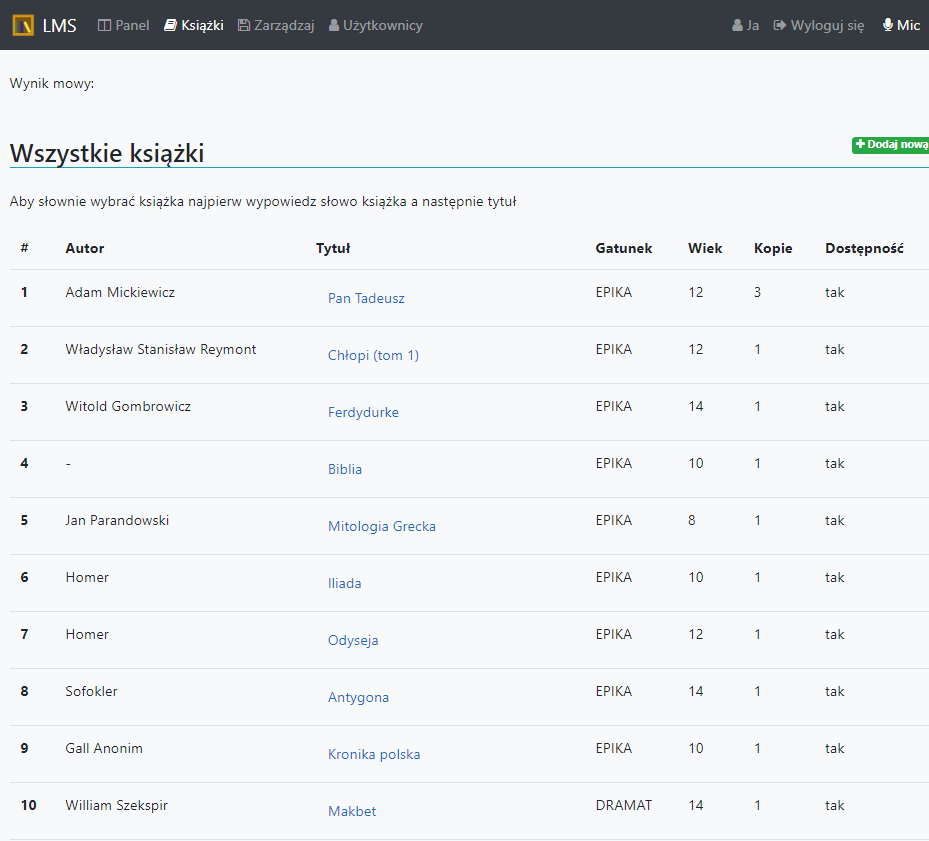
\includegraphics[width=\textwidth]{images/books}
        \captionsource{Ekran Książki}{Opracowanie własne}
        \label{fig:book}
    \end{subfigure}
    \hfill
    \begin{subfigure}[b]{0.4\textwidth}
        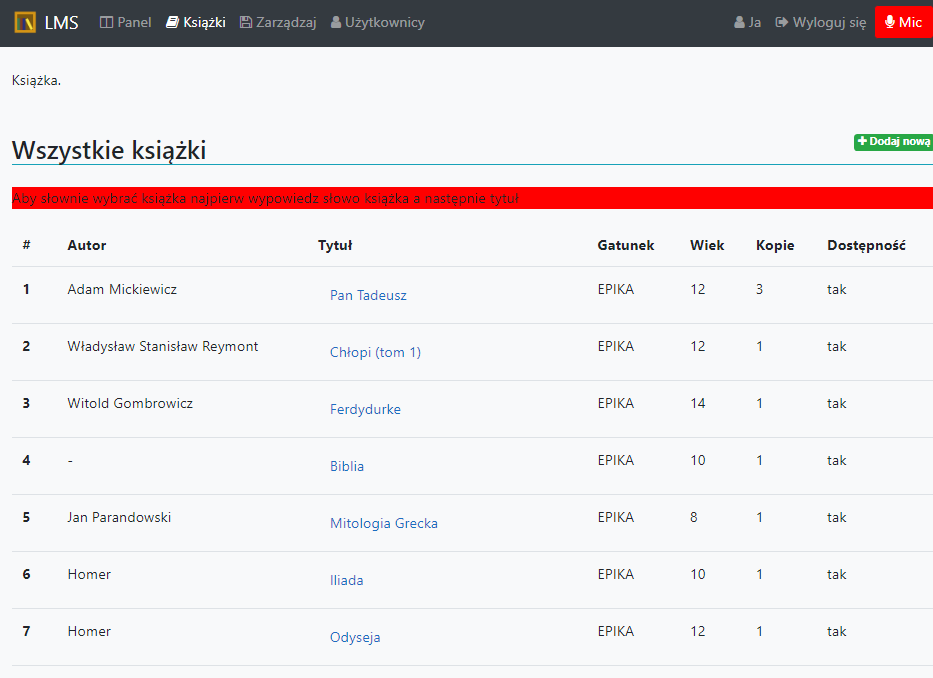
\includegraphics[width=\textwidth]{images/book1}
        \captionsource{Ekran Książki po wypowiedzeniu słowa książka}{Opracowanie własne}
        \label{fig:book1}
    \end{subfigure}
    \captionsource{Książki}{Opracowanie własne}
    \label{fig:book-oss}
\end{figure}

Po przejściu do ekranu pozwalającego dodać nową książkę użytkownik zostaje poproszony o wypełnienie krótkiego formularza w którym zawarte są podstawowe informacje o nowej pozycji tak jak to zostało przedstawione na \refsource{rysunku}{fig:addbook}.\ Operacje dodania książki można wykonać również w sposób głosowy, podając etykiety pól formularza a następnie wypowiadając to co ma się w danym polu znajdować.


\begin{figure}[H]
    \centering
    \begin{subfigure}[b]{0.4\textwidth}
        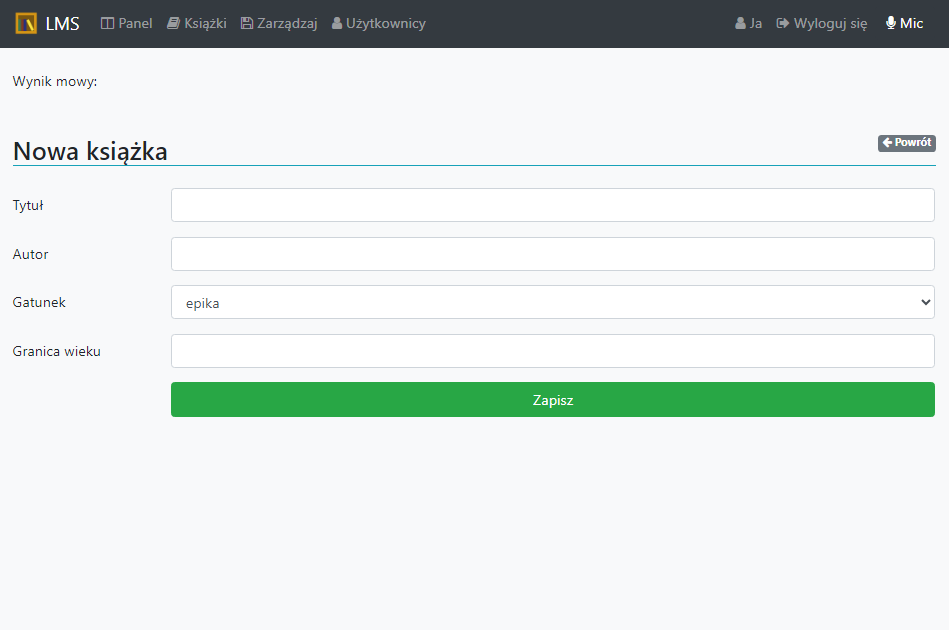
\includegraphics[width=\textwidth]{images/addBook}
        \captionsource{Formularz dodawania książek}{Opracowanie własne}
        \label{fig:addbook}
    \end{subfigure}
    \hfill
    \begin{subfigure}[b]{0.4\textwidth}
        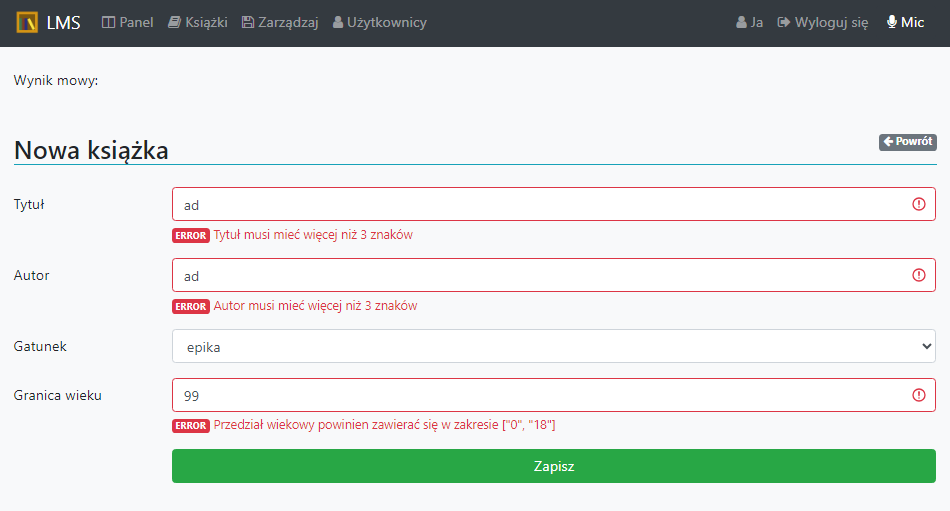
\includegraphics[width=\textwidth]{images/badaddBook}
        \captionsource{Formularz wypełniony błędnie}{Opracowanie własne}
        \label{fig:addbookbad}
    \end{subfigure}
    \captionsource{Dodawanie książek}{Opracowanie własne}
    \label{fig:book-oooadad}
\end{figure}

Jeśli po zapisaniu formularza nastąpi błąd.\ Błędne pola zostaną podkreślone, a błędy zostaną wypisane i powiedziane (z wykorzystaniem syntezatora mowy) przez formularz.\ Wygląd błędnego formularza został ukazany na \refsource{ekranie}{fig:addbookbad}.\ Po poprawnym wypełnieniu i zapisaniu formularza zostanie dodana nowa książka.\ Panel informacyjny o książce został wskazany na \refsource{obrazku}{lib:booki}.\ Na tym ekranie dostępne są podstawowe informacje na temat książki oraz informacje o jej wypożyczeniach.\ Z zaprezentowanego \refsource{ekranu}{lib:booki} jest możliwość zarządzać samą książką.

\begin{figure}[H]
    \centering
    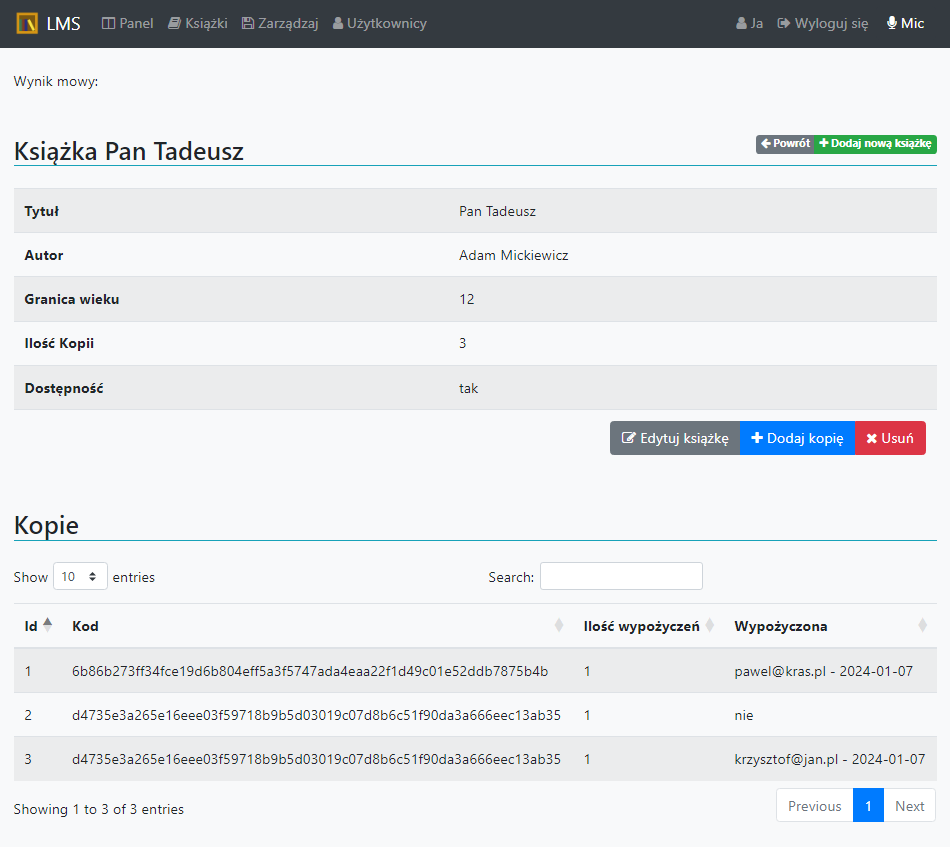
\includegraphics[width=0.4\textwidth]{images/infobook}
    \captionsource{Ekran informacyjny o książce}{Opracowanie własne}
    \label{lib:booki}
\end{figure}


\section{Zarządzaj}
Ekran ''\textit{Zarządzaj}'' pozwala na zarządzanie listą wypożyczeń oraz dostępnych książek.\ Dodatkowo jest to też wyszukiwarka, która pozwala na wyszukiwanie konkretnych tytułów.\ Został on przedstawiony na \refsource{zdjęciu}{fig:zaz}.\ Ekran pozwala na wypożyczanie oraz oddawanie książek.\ Można tą operację wykonać również głosowo po wypowiedzeniu słowa ''\textit{indeks}'', co zaznaczy kolumnę i poczeka na wypowiedzenie numeru indeksu tak jak na \refsource{rysunku}{fig:zaz1}.\ Aby oddać książkę należy wybrać przycisk ''\textit{Oddaj}'', bądź wypowiedzieć nazwę indeksu z tym przyciskiem.

\begin{figure}[H]
    \centering
    \begin{subfigure}[b]{0.4\textwidth}
        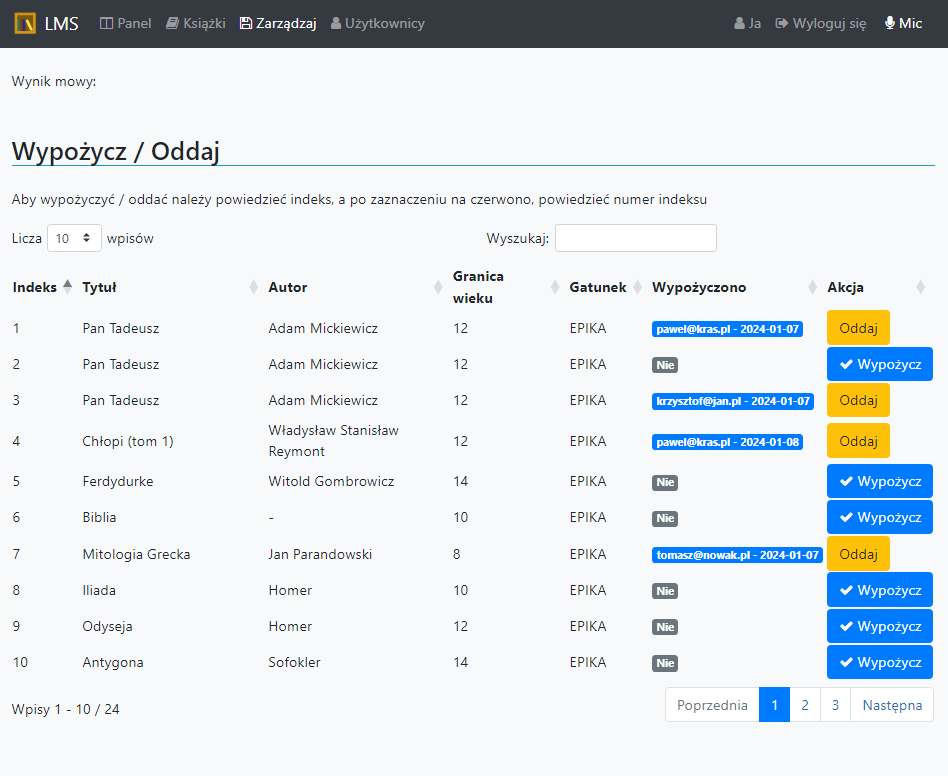
\includegraphics[width=\textwidth]{images/zaz}
        \captionsource{Ekran Zadządzaj}{Opracowanie własne}
        \label{fig:zaz}
    \end{subfigure}
    \hfill
    \begin{subfigure}[b]{0.4\textwidth}
        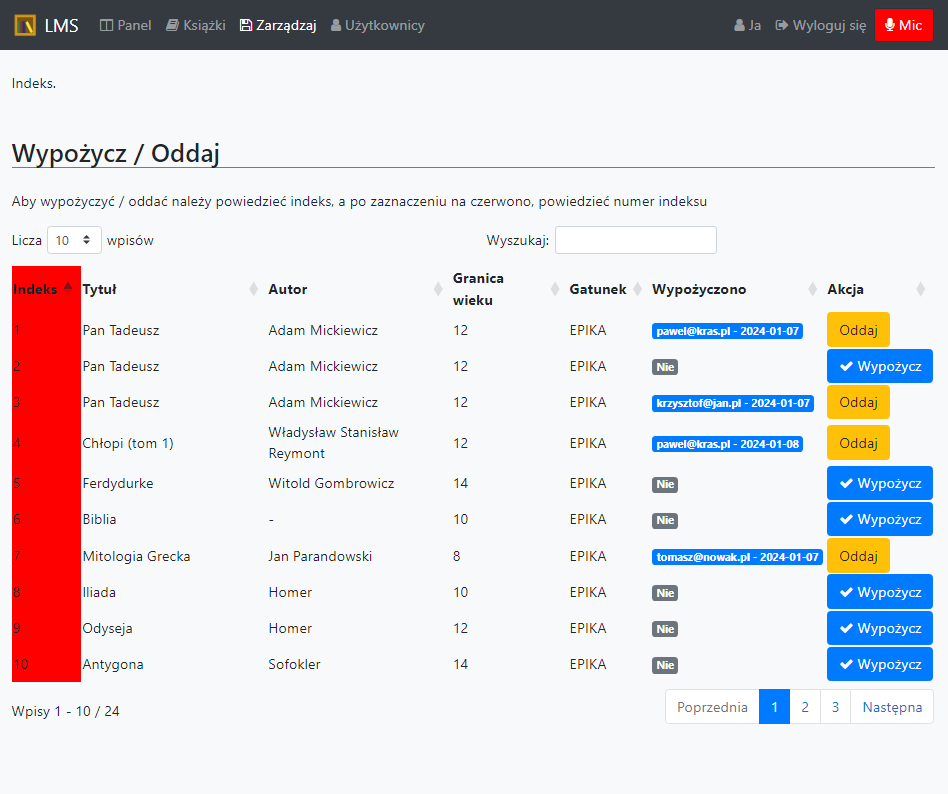
\includegraphics[width=\textwidth]{images/ind}
        \captionsource{Ekran z zaznaczoną kolumną Indeks}{Opracowanie własne}
        \label{fig:zaz1}
    \end{subfigure}
    \captionsource{Ekran Wypożyczenia}{Opracowanie własne}
    \label{fig:book-ooo}
\end{figure}

Aby wypożyczyć należy zrobić czynność analogiczną ale dla słowa ''\textit{Wypożycz}''. Dodatkowo po wybraniu przycisku ''\textit{Wypożycz}'' użytkownik zostanie przekierowany na odpowiedni ekran, który został ukazany na \refsource{zdjęciu}{fig:new}. Tam należy wskazać odpowiedniego użytkownika i kliknąć ''\textit{Zapisz}''.

\begin{figure}[H]
    \centering
    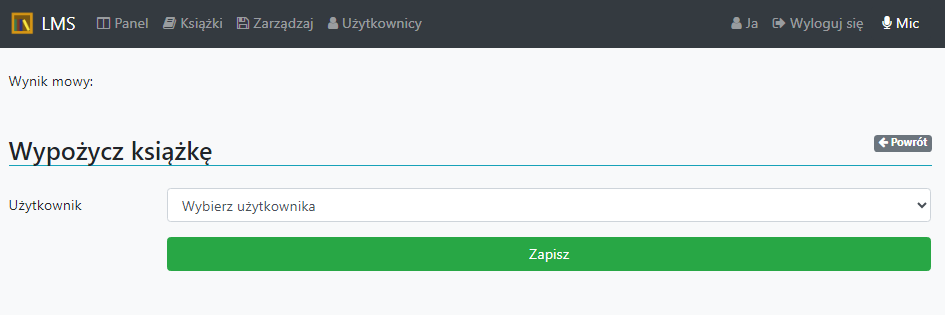
\includegraphics[width=0.4\textwidth]{images/new}
    \captionsource{Ekran wypożyczenia}{Opracowanie własne}
    \label{fig:new}
\end{figure}

\section{Użytkownicy}
Kolejnym panelem jest panel ''\textit{Użytkownicy}'', który pozwala na zarządzanie użytkownikami.\ Główne okno prezentuje listę użytkowników z możliwością dodania nowego użytkownika oraz zobaczenia informacji o użytkowniku. \refsource{Rysunek}{fig:us} pokazuje listę użytkowników Z możliwością wyszukiwania po niej.\ \refsource{Obraz}{fig:us1} pokazuje okno informacyjne o użytkowniku, a \refsource{ekran}{fig:us2} pokazuje formularz dodania nowego użytkownika.

\begin{figure}[H]
    \centering
    \begin{subfigure}[b]{0.3\textwidth}
        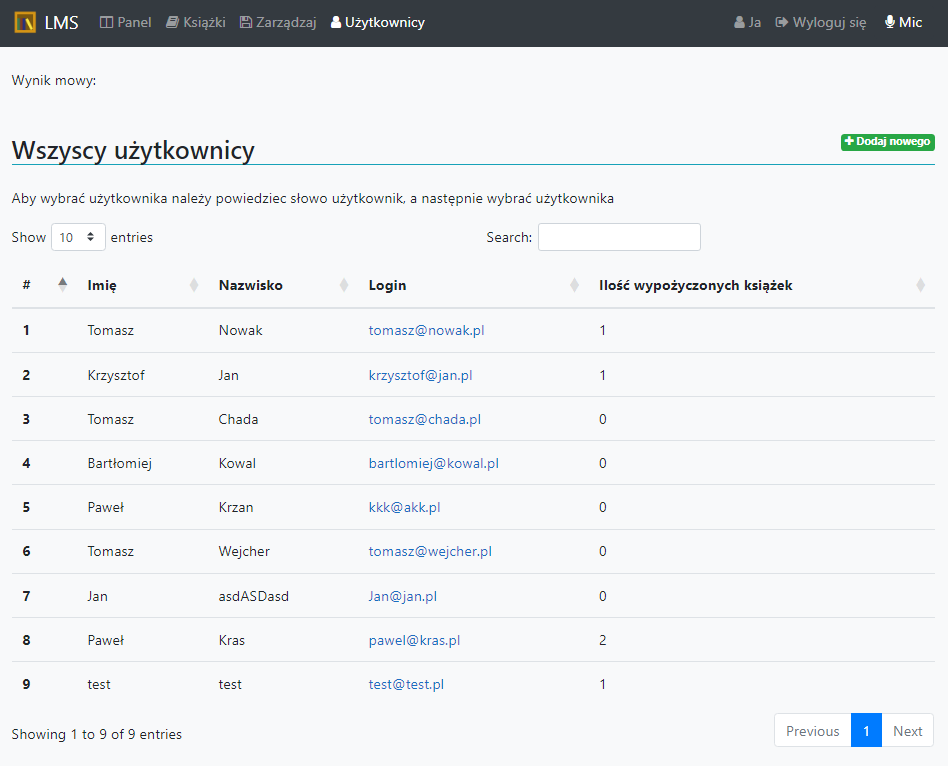
\includegraphics[width=\textwidth]{images/us}
        \captionsource{Ekran Użytkownicy}{Opracowanie własne}
        \label{fig:us}
    \end{subfigure}
    \hfill
    \begin{subfigure}[b]{0.3\textwidth}
        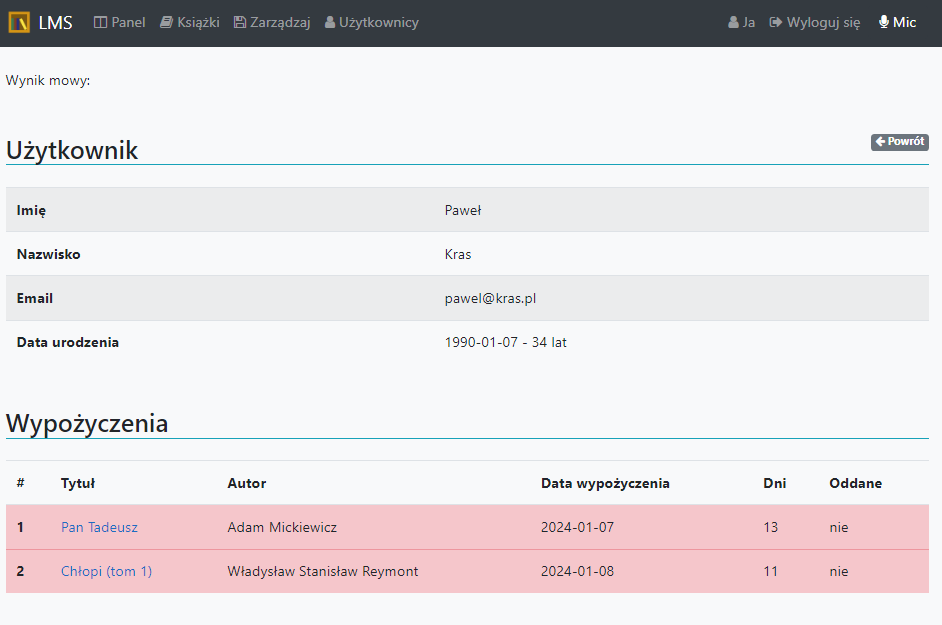
\includegraphics[width=\textwidth]{images/us1}
        \captionsource{Ekran informacyjny}{Opracowanie własne}
        \label{fig:us1}
    \end{subfigure}
    \hfill
    \begin{subfigure}[b]{0.3\textwidth}
        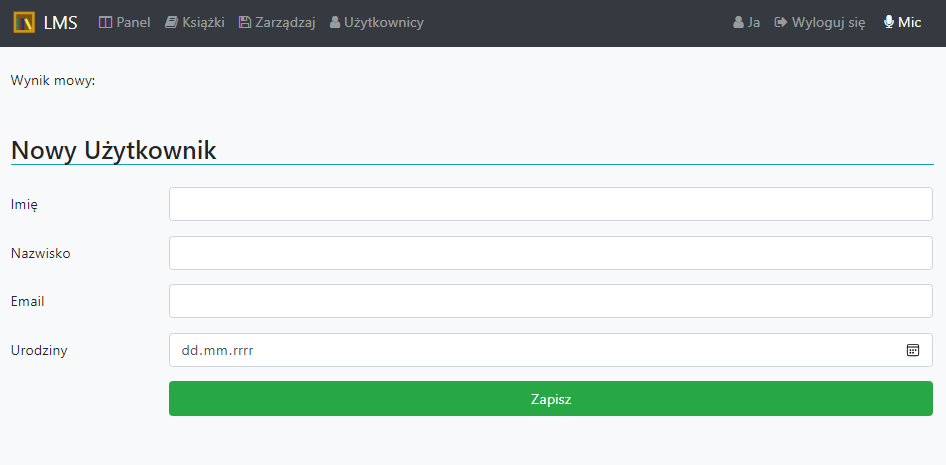
\includegraphics[width=\textwidth]{images/us2}
        \captionsource{Formularz użytkownika}{Opracowanie własne}
        \label{fig:us2}
    \end{subfigure}
    \captionsource{Użytkownicy}{Opracowanie własne}
    \label{fig:userrrrr}
\end{figure}

\section{Ja}
Ostatnim panelem jest ekran z informacjami zalogowanego użytkownika, pokazany na \refsource{rysunku}{fig:ja}.\ Pozwala on na sprawdzenie informacji o koncie oraz ich zmodyfikowaniu za pomocą formularza pokazanego na \refsource{zdjęciu}{fig:ja1}.

\begin{figure}[H]
    \centering
    \begin{subfigure}[b]{0.4\textwidth}
        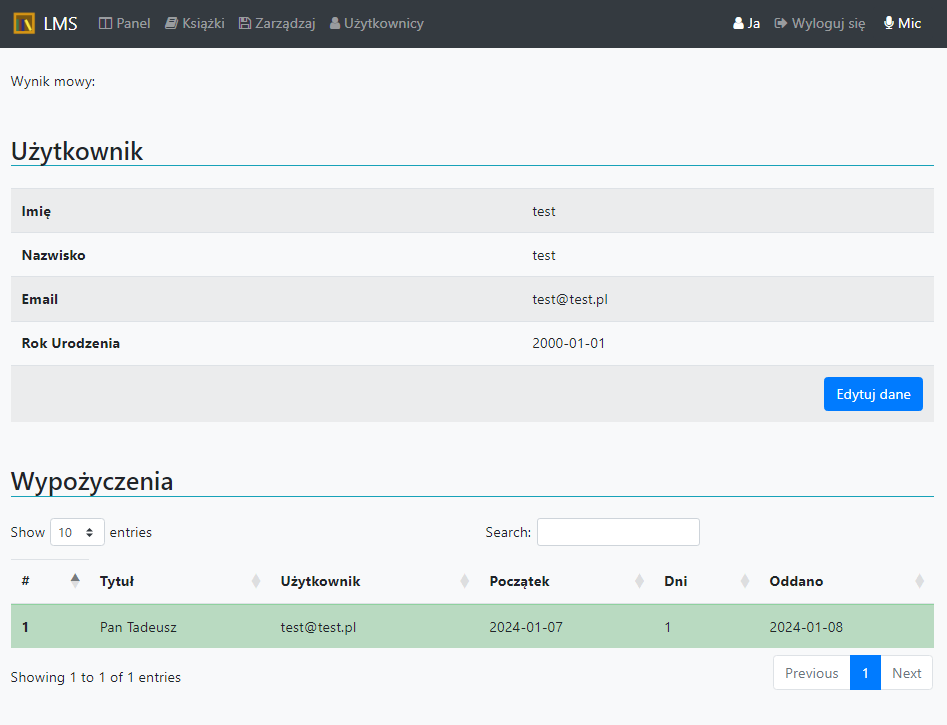
\includegraphics[width=\textwidth]{images/ja}
        \captionsource{Ekran Ja}{Opracowanie własne}
        \label{fig:ja}
    \end{subfigure}
    \hfill
    \begin{subfigure}[b]{0.4\textwidth}
        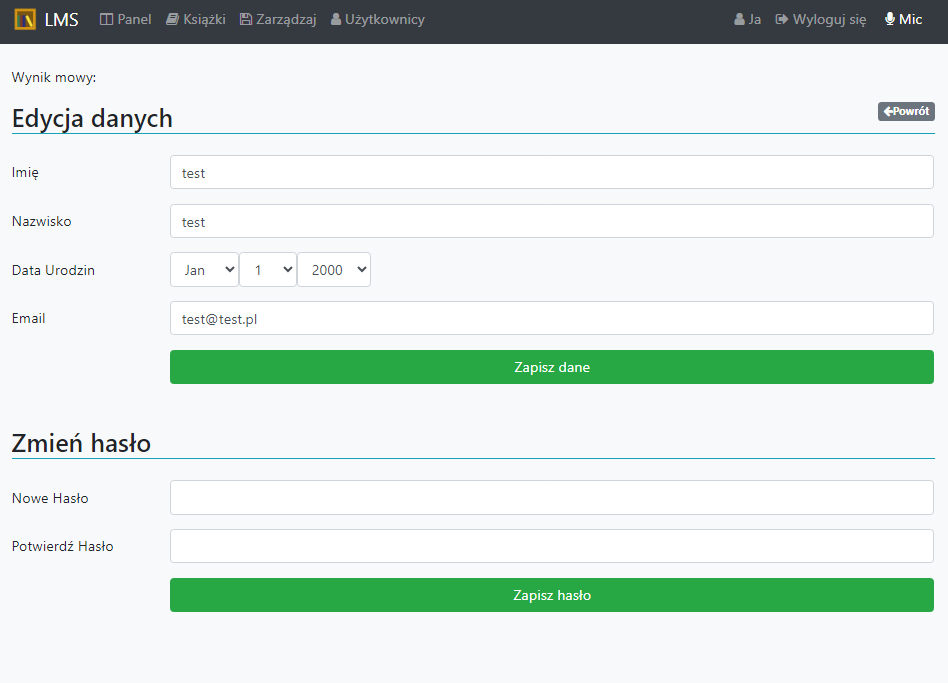
\includegraphics[width=\textwidth]{images/ja1}
        \captionsource{Formularz modyfikacji danych}{Opracowanie własne}
        \label{fig:ja1}
    \end{subfigure}
    \captionsource{Ekran o mnie}{Opracowanie własne}
    \label{fig:meeeee}
\end{figure}